\documentclass{article}
\usepackage{float}
\usepackage{tabto}
\usepackage{graphicx}
\usepackage[utf8]{vietnam}
\usepackage{caption}
\title{\textbf{MaSSP AI PROJECT DAILY REPORT NO. 4}}
\author{textbf{Team 3}\\
Nìm Trí Nghĩa\\
Hồ Chí Vương\\
Nguyễn Khắc Minh
}
\date{Thursday, July 11th, 2019}


\begin{document}
\maketitle
\textit{Project theme: OBJECT DETECTION – Finding certain objects from input images or videos} 
\graphicspath{ {./images/} }

\section{General Progress}
\begin{itemize}
	\item{Created a GUI for our video detecting app.}
	\item{Close to launching a local website}
	\item{added final touches and shaved off redundant codes}
	\item{Test-ran and debugged the entire program.}
\end{itemize}

\subsection{GUI}
We have created an interface mainly from the OpenCV library. The GUI comprises a camera button and currently 3 (we will be implementing more models) options to detect on video. 

\begin{figure}[h!]
	\includegraphics[scale=0.7]{GUI.PNG}
	\caption*{Image 1: New GUI}
	\label{GUI}
\end{figure}

\subsection{Website}
Due to our team's inexperience with coding websites, we had to ask for much help from our mentors, especially mentor Hiếu. We learned that to launch our website online, we have to be well-versed in not only coding Java and Html, but also in other things like legal matters...; and so we had to abandon that idea. However, since we have already started, we will settle with a local website.

\subsection{final program}
After a week of research and coding, we have been able to create both a  light-weight photo detector and a live recording detector, all wrapped-up in a simple app. We had both features implemented for the sake of not limiting the app function to high-end devices (since the live video detector is relatively demanding).

\section{Obstacles}
\begin{itemize}
	\item{Lack of experience in coding websites cost us a lot of time}
	\item{We only have one laptop powerful enough to run the video detector at a moderately bearable frame-rate, meaning that only one of us can debug and work on the code at any given time}
\end{itemize}

\begin{figure}[h!]
	\centering
	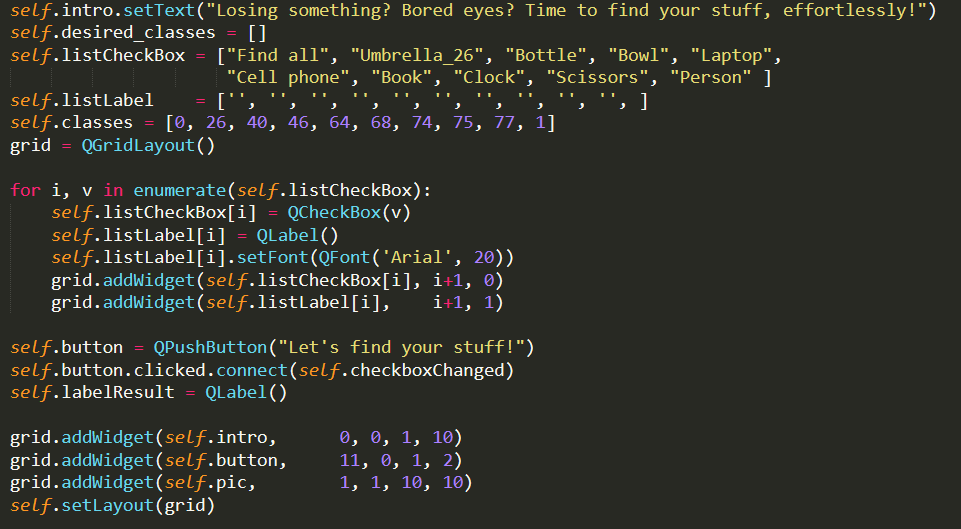
\includegraphics[scale=0.7]{demo.PNG}
	\caption*{image 2: code demo of GUI}
\end{figure}


\section{Future Plan}
\begin{itemize}
	\item Show-casing our program on tomorrow's mock presentation
	\item finishing our technical report, detailing how the model works
	\item Finishing off our website and possibly adding it to the final presentation
\end{itemize}

\end{document}
	 
